\documentclass{article}	% essential first line
\usepackage{float}		% this is to place figures where requested!
\usepackage{times}		% this uses fonts which will look nice in PDF format
\usepackage{graphicx}		% needed for the figures
\usepackage{url}
\usepackage{sbc-template} 
\usepackage[scaled]{uarial}


%% Here I adjust the margins

\oddsidemargin 0.1in		% Left margin is 1in + this value
\textwidth 6.25in		% Right margin is not set explicitly
\topmargin -0.2in			% Top margin is 1in + this value
\textheight 9in			% Bottom margin is not set explicitly
\columnsep 0.25in		% separation between columns

%% Define a macro for inserting postscript images
%% ==============================================
%% This is a macro which nominally takes 3 parameters, 
%% it would be used as follows to insert and encapsulated postscript
%% image at the location where it is used.
%%
%% \EPSFIG{epsfilename}{caption}{label}
%% - epsfilename is the name of the encapsulated postscript file to be
%%               inserted at this location
%% - caption is the text to be shown as the figure caption, it will be
%%           prepended by Figure X.  The number X can be referenced
%%           using the label parameter.
%% - label is a name given to the figure, it can be referenced using the
%%         \ref{label} command.

\def\EPSFIG[#1]#2#3#4{		% Don't be scared by this monsrosityok
\begin{figure}[H]		% it is a macro to save typing later
\begin{center}			% 
\includegraphics[#1]{#2}	%
\end{center}			%
\caption{#3}			%
\label{#4}			%
\end{figure}			%
}				%


%% Define the fields to be displayed by a \maketitle command\includegraphics[]{underreported.pdf}

\sloppy
\author{Felipe M. Besson \\ Pedro M. B. Leal}
\title{\begin{huge}\textbf{User Guide}\end{huge} \\ Baile V\&V Prototype}
 
\address{Department of Computer Science \\ Institute of Mathematics and Statistics\\
University of S\~ao Paulo (USP) 
\email{\{besson,pedrombl\}@ime.usp.br} }


\begin{document}	
\maketitle			

\date 

\newpage
\section { Overview }
This software prototype is part of HP Baile Project\footnote{Baile Project: http://ccsl.ime.usp.br/baile/}, more specifically, 
this prototype belongs to the research line ``Verification \& Validation of Choreographies''. More details about this research line and the
basis of our software can be found in this technical report~\cite{tech-report}. Our prototype are composed by:

\begin{itemize}
 \item a web service choreography developed on OpenKnowledge(OK)\footnote{OpenKnowledge: http://www.openk.org/};
 \item JUnit test cases developed for the coreography testing
 \item \textit{Ad hoc} scripts for enacting and testing the choreography automated
\end{itemize}

In this user guide, we described in steps how to install and use the software.


\section{ Prerequisites}
The following software elements must be installed and working:

\begin{itemize}
 \item Java 6~\cite{java6}
 \item SQLite 3~\cite{sql3}
 \item Ant~\cite{ant}
\end{itemize}

\section{ Where to download ? }
The prototype can be download in: XXXXXXX. The source code of the web services used and the REST client can also be available on the CCSL repository: YYYYYYYYY. 


\section{ Software directory structure}
Our prototype are structure in the following files and directories (just the most important are described bellow):

 \begin{table}[htb]
  \centering
  \begin{tabular}{|l|l|}
  \hline
  file/directory & Description \\
  \hline
  \hline
  baile.sh & script to start the application \\
  src/ & source code \\
  test/ & test code \\
  config/ & OpenKnowledge configuration files \\
  lcc/ & OpenKnowledge interaction model \\
  lib/ & third-party dependencies \\
  log/ & log files \\
  test-reports/ & html test reports \\
  \hline
  \end{tabular}
  \end{table}

\newpage 

\section{ How to use ? }
In this section, we detailed the main steps to interact with the application.

\begin{enumerate}
 \item Start the script \textbf{baile.sh}, and then, the application will start:

  \begin{figure}[htbp]
  \centering
  \setlength\fboxrule{1.0pt}
  \scalebox{0.5}{\fbox{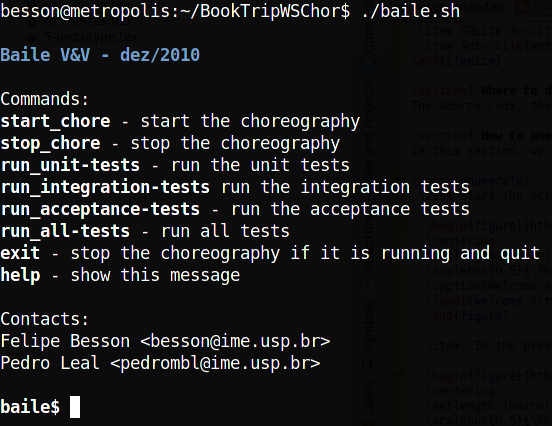
\includegraphics{fig/welcome-screen}}}
  \caption{Welcome screen}
  \label{welcome-screen}
  \end{figure}

  \item  In the prompt, start the choreography by typing \textbf{start\_chore} (as showed in Figure~\ref{chore})
  
  \begin{figure}[htbp]
  \centering
  \setlength\fboxrule{1.0pt}
  \scalebox{0.5}{\fbox{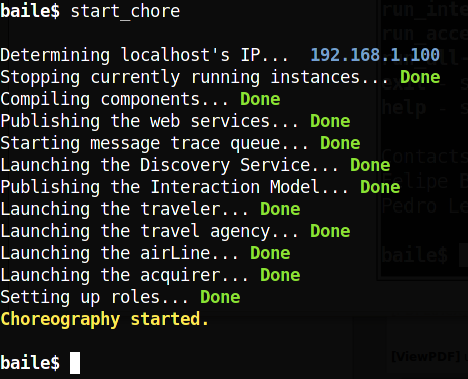
\includegraphics{fig/chore}}}
  \caption{Starting the choreography}
  \label{chore}
  \end{figure}

  \item Once all components of choreography (services, roles, OpenKnowledge entities) have been started successfully (as showed in Figure~\ref{chore}), the tests can be execute. The following commands are valid:

  \begin{table}[htb]
  \centering
  \begin{tabular}{|l|l|}
  \hline
  Command & Description \\
  \hline
  \hline
  run\_unit-tests & run the unit tests\\
  run\_integration-tests & run the integration tests \\
  run\_acceptance-tests & run the acceptance tests \\
  run\_all-tests & run all tests \\
  \hline
  \end{tabular}

  \end{table}

\end{enumerate}


\section{ How to add more test cases ? }
The script compiles every test class of the test folder before any test execution. So, modifications on a existing test class, will be compiled before the next command tests executed.

Any new test class need to be added in its test strategy folder (unit, integration, or acceptance). After the addition, the script will recognised the new class automatically. 

\section{ Known Issues }
Our choreography does not support interactions interruptions properly. So, if any test was forced interrupted, in some cases, the choreography must be restarted. There are some crash but rare communication errors. When these erros happened, the processes that compose the choreography must be killed. It can be done executing the script \textit{./script/stopChor.sh}. 

\section{Acknowledgements}
This research received funding from HP Brasil under the Baile Project.


\newpage
\bibliographystyle{abbrv}	% Order by citation
\bibliography{references}

\end{document}

